\documentclass[conference]{IEEEtran}
\IEEEoverridecommandlockouts
% The preceding line is only needed to identify funding in the first footnote. If that is unneeded, please comment it out.
\usepackage{cite}
\usepackage{amsmath,amssymb,amsfonts}
\usepackage{algorithmic}
\usepackage{graphicx}
\usepackage{textcomp}
\usepackage{xcolor}
\def\BibTeX{{\rm B\kern-.05em{\sc i\kern-.025em b}\kern-.08em
    T\kern-.1667em\lower.7ex\hbox{E}\kern-.125emX}}
\begin{document}

\title{Multi-Agent Reinforcement Learning Benchmark on Highway Environment for Autonomous Driving\\}


\author{\IEEEauthorblockN{Charbel Abi Hana}
\IEEEauthorblockA{\textit{M1 International Track in Electrical Engineering} \\
\textit{Université Paris-Saclay}\\
Paris, France \\
charbel-a-h@outlook.com}
}

\maketitle

\begin{abstract}
The rise of deep learning paved the way for the development of deep Reinforcement Learning methods in control, navigation and autonomous driving.
The domain of Reinforcement Learning (RL) has become a powerful learning framwork capable of learning complex policies in high-dimensional environments. In this research project
we aim to benchmark some of the widely used deep reinforcement learning methods on a simulated multi-agent highway environment. We will benchmark two decentralized algorithms; \textbf{IDQN} and \textbf{IPPO} 
which will control autonmously driven vehicles in a high density and high speed highway full of road (human driven) vehicles.  
\end{abstract}

\begin{IEEEkeywords}
Reinforcement Learning, Autonomous Driving, IDQN, IPPO
\end{IEEEkeywords}

\section{Introduction}
Autonomous driving systems constitute of multiple perception level tasks that have now achieved high precision on account of deep learning architectures. 
Besides the perception, autonomous driving systems constitute of multiple tasks where classical supervised 
learning methods are no more applicable. First, when the prediction of the agent's action changes future 
sensor observations received from the environment under which the autonomous driving agent operates, for 
example the task of optimal driving speed in an urban area. Second, supervisory signals such as time 
to collision, lateral error with respect to optimal trajectory of the agent, represent the dynamics of the 
agent, as well uncertainty in the environment. Such problems would require defining the stochastic cost 
function to be maximized. Third, the agent is required to learn new configurations of the environment, as 
well as to predict an optimal decision at each instant while driving in its environment. 
This represents a high dimensional space given the number of unique configurations under which the agent and environment are observed, this is combinatorially
large. In such cases, we will solve the decision making process by formalizing it under the classical settings of Reinforcement Learning where an agent is required
to optimally act in a given environment given a representation of that environment at a certain time step. The optimal set of actions taken by the agent is called the policy.
In this research project, we will define the basic building blocks of a Reinforcement Learning algorithm, provide two implementations of those algorithms which leverage deep learning
through multi-layered perceptron or convolution neural networks like the \textbf{IDQN} and \textbf{IPPO} which are direct extensions of the well-known Deep-Q-Learning (DQN\cite{https://doi.org/10.48550/arxiv.1312.5602}) and Proximal Policy Optimization (PPO\cite{https://doi.org/10.48550/arxiv.1707.06347}) respectively on a multi-agent level.
The performance of each algorithm will be tested on an OpenAI Gym environment called \textit{Highway-env} which simulates real world driving on an n-lane highway.

\section{Background}

\subsection{Reinforcement Learning}

\begin{figure}[htbp]
\centerline{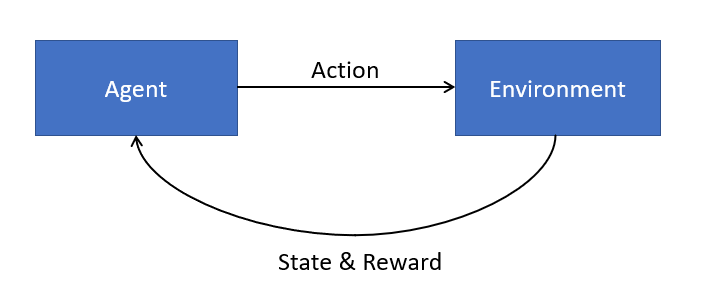
\includegraphics[width=60mm]{images/rl_diag.png}}
\caption{Generated Output after 50 Epochs}
\label{fig5}
\end{figure}

\subsection{Multi-Agent Reinforcement Learning}

\subsection{Deep Q-Learning}

\begin{figure}[htbp]
\centerline{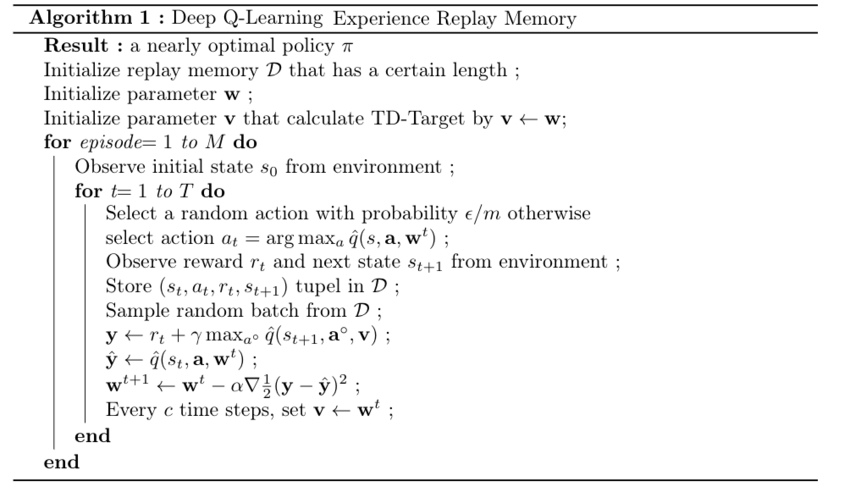
\includegraphics[width=80mm]{images/DQN-Algorithm.png}}
\caption{Deep Q-Learning Algorithm}
\label{fig4}
\end{figure}

\subsection{Proximal Policy Optimization}

\begin{figure}[htbp]
\centerline{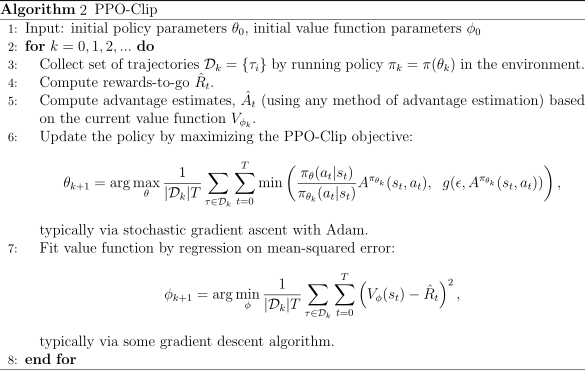
\includegraphics[width=80mm]{images/ppo_algorithm.png}}
\caption{Proximal Policy Optimization Algorithm}
\label{fig6}
\end{figure}

\begin{equation}
\min_{G}\max_{D}\mathcal V_{\text{GAN}}\left(D, G \right) = \end{equation}
\begin{align*}
 \mathbb E_{x \sim p_{\text{data}\left( x\right) }}\left[ \log \left\{ D\left( x \right) \right\} \right] + \mathbb E_{z\sim p_{z}\left( z\right)}\left[ \log\left\{ 1 - D\left( G\left( z\right) \right) \right\}\right].   
\end{align*}

where \begin{math}G : R^{100} \longrightarrow R^{16,384}\end{math}
\begin{equation}
L_D = - \sum_{x \in \chi, z \in \zeta} \log(D(x)) + \log(1 - D(G(z))) \tag{6}
\end{equation}
\begin{equation}
L_G = - \sum_{z \in \zeta} \log(D(G(z)) \tag{7}
\end{equation}


\begin{equation}
h^{[i]} = LeakyRELU(W^{[i-1]}h^{[i-1]}+b{[i-1]})\label{Gen LeakyRELU}
\end{equation}
\begin{math}\alpha \end{math}, with h[i] \begin{math}\epsilon R^{16\alpha2^i}\end{math} and we output the vector o \begin{math}\epsilon R^{16,384}\end{math} via
\begin{equation}
o =\tanh(W^{[L]}h^{[L]}+b{[L]})
\end{equation}
Where L is the final layer.

\begin{math}h[0]\end{math} denote the input
image, \begin{math}W [j]\end{math} and \begin{math}b[j]\end{math} denoting the weight matrix and the bias vector in the L output layer, we have:
\begin{equation}
o = sigmoid(W^{[L]}h^{[L]}+b{[L]})
\end{equation}


\section{Environment}

\begin{figure}
\centerline{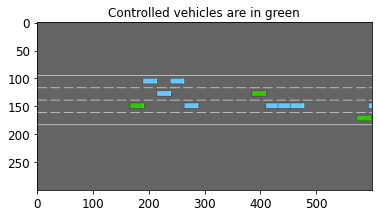
\includegraphics[width=75mm]{images/highway-env.png}}
\caption{Random Cows and Horses Images from Original Dataset}\label{fig1}
\end{figure}

\subsection{Action Space}

\begin{figure}
\centerline{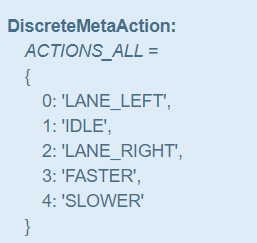
\includegraphics[width=0.3\linewidth]{images/action_space.png}}
\caption{Generated Output after 100 Steps}
\label{fig2}
\end{figure}

\subsection{Observation Space}

\begin{figure}
\centerline{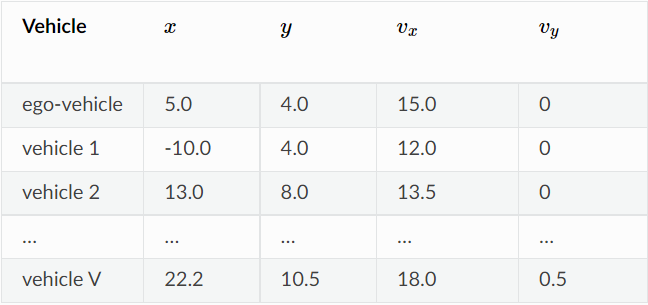
\includegraphics[width=80mm]{images/observation_space.png}}
\caption{Generated Output after 35000 Steps}
\label{fig3}
\end{figure}

\subsection{Reward}


\section{Experimentation and Results}

\subsection{Evaluation Metrics}


\subsection{Results}


\begin{table}[h!]
\centering
\begin{tabular}{| *{9}{c|} }
    \hline
\textbf{Metric}    & \multicolumn{2}{c|}{Orig}
            & \multicolumn{2}{c|}{Orig-250-GAN}
                    & \multicolumn{2}{c|}{Orig-500-GAN}
                            & \multicolumn{2}{c|}{Orig-1000-GAN}                \\
    \hline
-   &   \textbf{train}  &   \textbf{val}  &   \textbf{train}  &   \textbf{val}  &   \textbf{train}  &   \textbf{val}  &   \textbf{train}  &   \textbf{val}  \\
    \hline
BCE-Loss   &   0.01  &   5  &   0.01  &   0.7  &  0.01   &  0.7   &   8  &  0.7   \\
    \hline
Accuracy   &    1.0   &     0.5  &   1.0    &     0.6  &   1.0    &    0.5   &   0.5    &   0.5    \\
    \hline
Precision   &   1.0    &   0.1    &   1.0    &    0.5   &   1.0    &    0.5   &   0.5    &    0.5   \\
    \hline
Recall   &    1.0   &    0.5   &    1.0   &   0.4   &    1.0   &    1.0   &    1.0   &  1.0     \\
    \hline

\end{tabular}
\caption{Compiled table of Classification Metrics}
\end{table}

\section{Conclusion}


\bibliographystyle{plain} % We choose the "plain" reference style
\bibliography{citations} % Entries are in the refs.bib file
\end{document}
